\documentclass[crop,tikz]{standalone}
\usetikzlibrary{backgrounds}
\colorlet{blue}{cyan}
\tikzset{
  inverted/.style = {
    color=white,
    background rectangle/.style={fill},
    show background rectangle
  }
}

\usepackage[european,americaninductors]{circuitikz}
\tikzset{>=latex}
\colorlet{green}{green}

\begin{document}
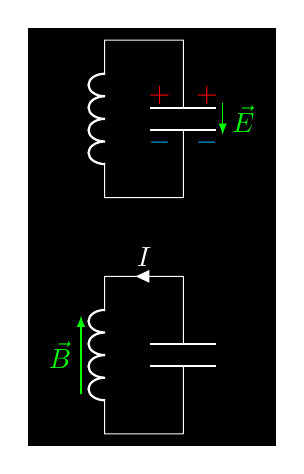
\begin{tikzpicture}[inverted,inverted]
  \draw (0,0) to ++(-1,0) to[L] ++(0,2) to ++(1,0) to[C] ++(0,-2);
  \node[red]  at (+0.3,1.3) {$+$};
  \node[red]  at (-0.3,1.3) {$+$};
  \node[blue] at (+0.3,0.7) {$-$};
  \node[blue] at (-0.3,0.7) {$-$};
  \draw[green,->] (0.5,1.2) -- node[right] {$\vec{E}$} ++(0,-0.4);
  %
  \draw (0,-3) to ++(-1,0) to[L] ++(0,2) to[short,i<={$I$}] ++(1,0) to[C] ++(0,-2);
  \draw[green,->] (-1.3,-2.5) -- node[left] {$\vec{B}$} ++(0,1);
\end{tikzpicture}
\end{document}
